% !TEX root = index.tex

\section{How Curved are Curves?}
\epigraph{The real problem in speech is not precise language. The problem is clear language.}{Richard Feynmann}
\subsection{Curvature of Curves}
Our first goal is to define a quantitative measure of curvature. For example, we would like to determine what the curvature of the sine curve is at various points. For us a \textbf{curve} $ C$ is the image of a smooth function $ c(t): (a,b) \rightarrow \R^2$ or $ \R^3$. The function $ c(t)$ is called a \textbf{parametrization} of the curve $ C$.
\begin{example} $ $
	\label{example:parametrizations}
	\begin{enumerate}
		\item The circle $ x^2 + y^2 = r^2$ can be parametrized as \begin{align*}
			      c(t) = (r \cos (\omega t), r \sin(\omega t))
		      \end{align*}
		      where $ \omega$ is any non-zero constant.
		\item The sine curve can be parametrized as
		      \begin{align*}
			      c(t) = (t, \sin t)
		      \end{align*}
		\item More generally, the graph $ y=f(x)$ can be parametrized as
		      \begin{align*}
			      c(t) = (t,f(t))
		      \end{align*}
	\end{enumerate}
\end{example}


\begin{figure}[H]
	\centering
	\begin{subfigure}[t]{0.4\textwidth}
		\centering
		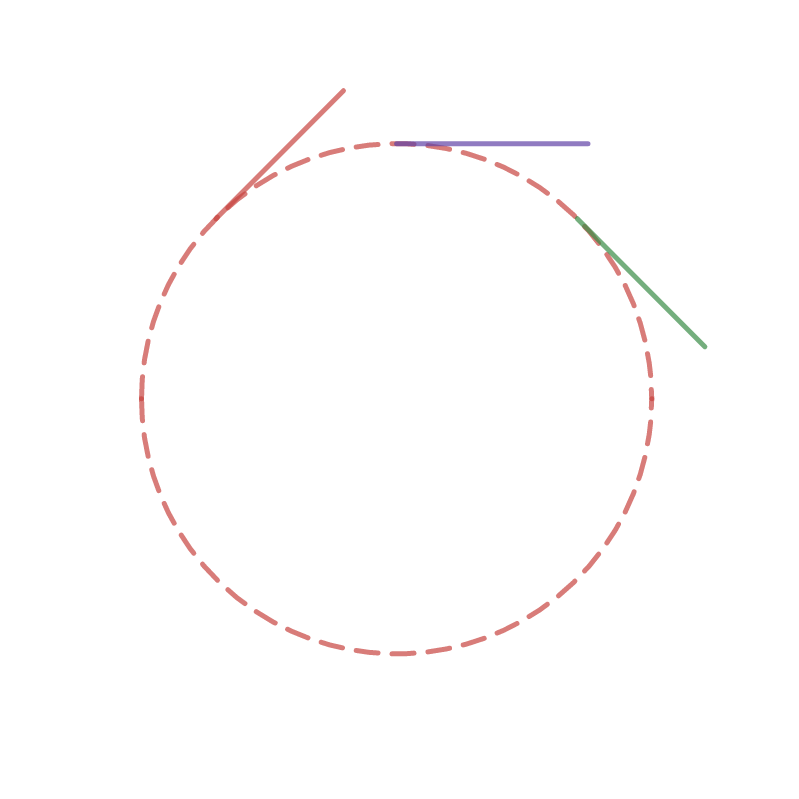
\includegraphics[height=6cm]{small_radius_circle}
	\end{subfigure}
	\begin{subfigure}[t]{0.59\textwidth}
		\centering
		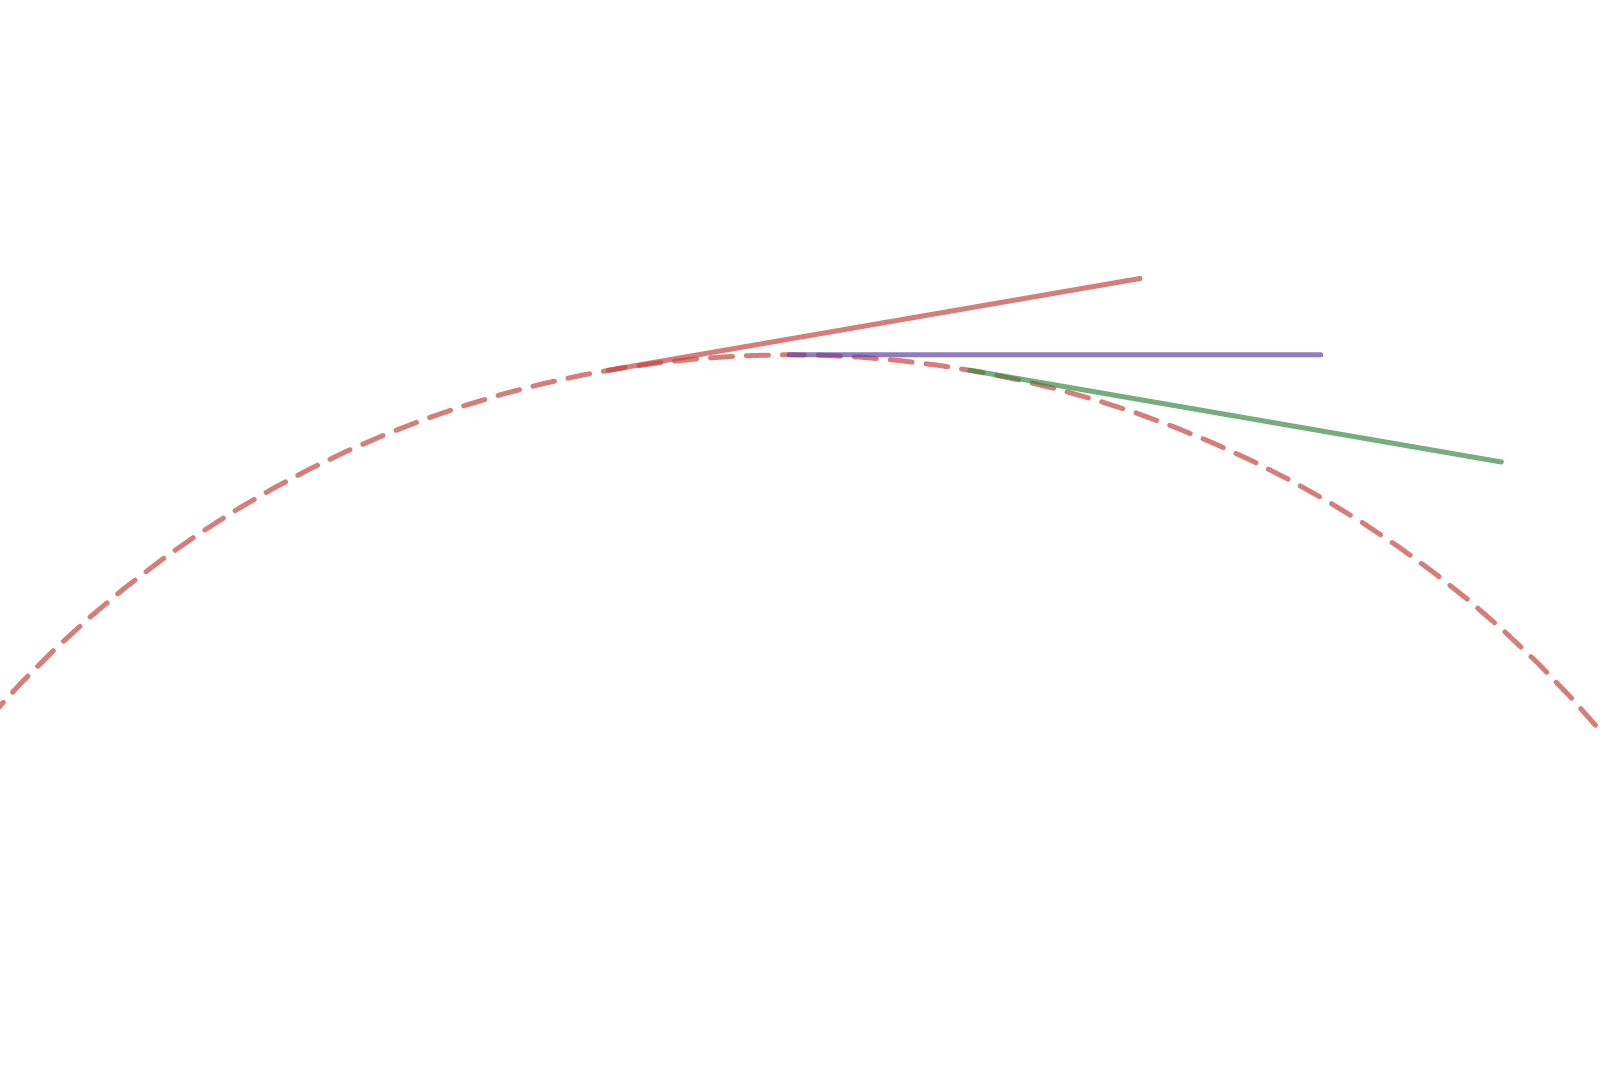
\includegraphics[height=6cm]{large_radius_circle}
	\end{subfigure}
	\caption{The smaller the radius of the circle the faster the rate of change of the tangent vector.}
\end{figure}

Recall that $ c'(t)$ is the \textbf{tangent vector} to the curve $ C$ at the point $ c(t)$. If a curve has large curvature then the angular component of the tangent vector should change rapidly as we move along the curve, conversely if a curve has small curvature then the angular component should change slowly, which suggests the following definition.

\begin{definition}
	The \textbf{curvature} $ \kappa$ of a curve $ C$ parametrized by $ c(t)$ is defined to be the rate of change of the angular component of $ c'(t)$.
\end{definition}
Recall that every non-zero vector $ \vec{v}$ can be written as $ \vec{v} = \norm{\vec{v}} . u$, where $ u$ is the unit vector in the direction of $ v$. The length $ \norm{\vec{v}}$ is the \textbf{radial component} of $ v$ and $ u = \vec{v} / \norm{\vec{v}}$ is the \textbf{angular component} of $ v$. We can make the above definition more precise as follows.
\begin{definition}
	The \textbf{curvature} of a curve $ C$ parametrized by $ c(t)$ is defined to be
	\begin{align*}
		\kappa
		&:= \mbox{ rate of change of the angular component of } c'(t) \\
		&= \left \lVert \dfrac{d}{dt} \left( \dfrac{c'(t)}{\norm{c'(t)}}\right) \right \rVert \cdot \dfrac{1}{\norm{c'(t)}}
	\end{align*}
	assuming $c'(t) \neq 0$.
\end{definition}
We divide by $\norm{c'(t)}$ to normalize the rate at which we're moving along the curve.
\begin{remark}
	It's not too hard to find parametrizations with $c'(t) \neq 0$, at least in a small neighborhood of the point under consideration. For example, all the examples in Example \ref{example:parametrizations} satisfy this condition (check this).
\end{remark}

From this definition we immediately get a way to compute the curvature in the special case when $ \norm{c'(t)}=1$ for all $ t$. Such a parametrization is called a \textbf{unit speed parametrization}.
\begin{prop}
For a unit speed parametrization $c(t)$ the curvature is given by
\begin{align*}
	\kappa
	&= \left \lVert \dfrac{d}{dt} \left({c'(t)}\right) \right \rVert = \norm{c''(t)}
\end{align*}
\end{prop}
\begin{example}
	A circle of radius $ r$ can be parametrized as
	\begin{align*}
		c(t) = (r \cos (\omega t), r \sin(\omega t))
	\end{align*}
	for some constant $ \omega$. For this parametrization
	$$\norm{c'(t)} = \norm{ (-r \omega \sin (\omega t), r \omega \cos(\omega t))} = r \omega $$
	If we choose $ \omega = 1/r$ the parametrization becomes unit speed. In this case the curvature equals
	\begin{align*}
		\kappa
		 & = \norm{c''(t)}                            \\
		 & = \norm{(r \cos (t/r), r \sin(t/r))}       \\
		 & = \norm{(-1/r \cos (t/r), -1/r \sin(t/r))} \\
		 & = \dfrac{1}{r}
	\end{align*}
:D
\end{example}

\begin{thm}
	The circle of radius $ r$ has constant curvature of $ 1/r$.
\end{thm}
It is not easy to find unit speed parametrizations for more complicated curves (try it out). We need a formula which is valid even for non-unit speed parametrizations.

\begin{thm}
	\label{thm:curvature_formula}
	The \textbf{curvature} of a curve $ C$ parametrized by $ c(t)$ is given by
	\begin{align*}
		\kappa = \dfrac{\norm{c'(t) \times c''(t)}}{\norm{c'(t)}^3}
	\end{align*}
	assuming $c'(t) \neq 0$.
\end{thm}
\noindent The proof is in the following exercise.
\begin{ques}
	Let $ c(t)$ be a parametrization of $ C$ which is not necessarily unit speed. Let $ r(t) = \norm{c'(t)}$ be the radial component of the velocity, suppose that $ r(t)$ is never 0. Let $ \theta(t) = c'(t)/ \norm{c'(t)}$ be the angular component of velocity. Note that $r(t)$ is a scalar valued function and $\theta(t)$ is a vector valued function. The curvature is given by
	\begin{align*}
		\kappa = \dfrac{\norm{\theta'(t)}}{r(t)}
	\end{align*}
	Use the following steps to compute $ \kappa$.
	\begin{enumerate}
    \item Express $c'(t)$ in terms of $r(t)$ and $\theta(t)$.
    \item Show that $ \theta'(t) \cdot \theta'(t)$ is a constant and equals 1.
		\item Show that $ \theta'(t) \cdot \theta''(t) = 0$ and hence $\theta'(t) \perp \theta''(t)$ for all $t$.
		\item Conclude that $ \norm{\theta'(t) \times \theta''(t)} = \norm{\theta''(t)}$.
		\item Express $ c''(t)$ in terms of $ r(t)$, $ \theta(t)$, and their derivatives.
		\item Prove Theorem \ref{thm:curvature_formula}.
	\end{enumerate}
\end{ques}
\begin{ques}
	Use the parametrization $(r \cos (\omega(t)), r \sin(\omega(t)))$ to compute the curvature of a circle of radius $r$, where now $\omega$ is a function of $t$.
\end{ques}
\begin{ques}
	An easy computation shows that curvature of the graph $y=x^4$ is 0 at $x=0$. What does this mean geometrically?
\end{ques}
\begin{ques} $ $
	\begin{enumerate}
		\item Find the curvature of the graph $y=f(x)$ where $f:\R \rightarrow \R$ is any smooth function.
		\item Guess the relationship between the curvature of the graphs $y=f(x)$ and $y=kf(x/k)$, where $k$ is a positive real number. Prove your guess.
		\item Guess the relationship between the curvature of curves parametrized by $c(t)$ and $kc(t)$, where $k$ is a positive real number. Prove your guess.
	\end{enumerate}
\end{ques}
The formula for curvature in Theorem \ref{thm:curvature_formula} explicitly depends on the parametrization $ c(t)$ but the curvature itself does not. Have you seen such phenomenon before? Perhaps in your favorite branch of mathematics?
\begin{remark}[Generalized Curvature]
	\label{remark:signed_curvature}
	Often in calculus, not taking absolute value or norm gives us quantities which do not have explicit geometric significance but are easier to manipulate. For example, the integral itself has no geometric significance rather the area under a curve is the \emph{absolute value} of the integral, however, the Fundamental Theorem of Calculus does not contain any absolute values. Analogously, we'll call the vector quantity
	\begin{align*}
		\vec{\kappa} := \dfrac{d}{dt} \left( \dfrac{c'(t)}{\norm{c'(t)}}\right) \cdot \dfrac{1}{\norm{c'(t)}}
	\end{align*}
the \textbf{Generalized Curvature} for the lack of a better name. The following theorem is the analogue of Fundamental Theorem of Calculus for Curvature.
\end{remark}
\begin{ques}
	For a curve $C$ with a parametrization $c(t)$ compute the integral
	\begin{align*}
		\int \limits_{t_0}^{t_1} \vec \kappa \: ds
	\end{align*}
	(Hint: Think about what this integral is computing geometrically. It might help to first solve this problem for a unit speed parametrization).
\end{ques}



\subsection{Curvature and Taylor approximation}

Let us now consider curves which are graphs $y=f(x)$. For simplicity we'll assume that 0 is a critical point of $f(x)$ i.e. $f'(0) = 0$, and that $f''(0) \ge 0$. The following theorem is an easy exercise.
\begin{thm}
  If $0$ is a the \textbf{critical point} of $f: \R \rightarrow \R$ then the curvature of the graph $y=f(x)$ at $(0,f(0))$ equals ${f''(0)}$.
\end{thm}
\begin{ques}
	Prove this.
\end{ques}
\noindent Thus the degree 2 Taylor approximation of $ f(x) $ at the critical point $ x=0$ is given by
\begin{align}
	\label{eq:eq2}
	\begin{split}
	f(x) &\approx f(0) + f''(0) \dfrac{x^2}{2} \\
  &=f(0) + \kappa \dfrac{x^2}{2}
\end{split}
\end{align}
There is another familiar function which has the same Taylor approximation. The equation of a circle of radius $ r$ centered at the origin in $ \R^2$ is $$ x^2 + y^2 = r^2 $$
\emph{Near} the point $(0,-r)$ we can express the circle as the graph $ y = -\sqrt{r^2 - x^2}$.
\begin{ques}
	Show that the degree 2 Taylor approximation of $ -\sqrt{r^2 - x^2} $ at $ x=0$ is given by
	\begin{align}
		\label{eq:eq1}
		-\sqrt{r^2 - x^2} & \approx -r + \dfrac{x^2}{2r}
	\end{align}
\end{ques}
Notice that $ 1/r$ which is the coefficient of $ x^2/2$ is exactly the curvature of the circle. We can interpret Equations \eqref{eq:eq1} and \eqref{eq:eq2} as saying that,
\begin{prop}
	\label{prop:approximating_circle}
	 If the curvature of the curve $ y=f(x)$ is $ \kappa$ at a critical point $p$ then \textbf{the circle that best approximates the curve at $p$ has radius $ 1/\kappa$}.
\end{prop}
Since we can always rotate a curve without changing it's curvature, Proposition \ref{prop:approximating_circle} is true in much more generality and we can drop the condition that $p$ is a critical point. We know from calculus that the first derivative gives us the slope of the tangent line. Here we are saying that the second derivative gives us the \emph{tangent} circle\footnote{The technical term is an \emph{osculating} circle.}.
\begin{ques}
	Think about how you might generalize the above methods to surfaces.
\end{ques}
\begin{figure}[H]
	\centering
		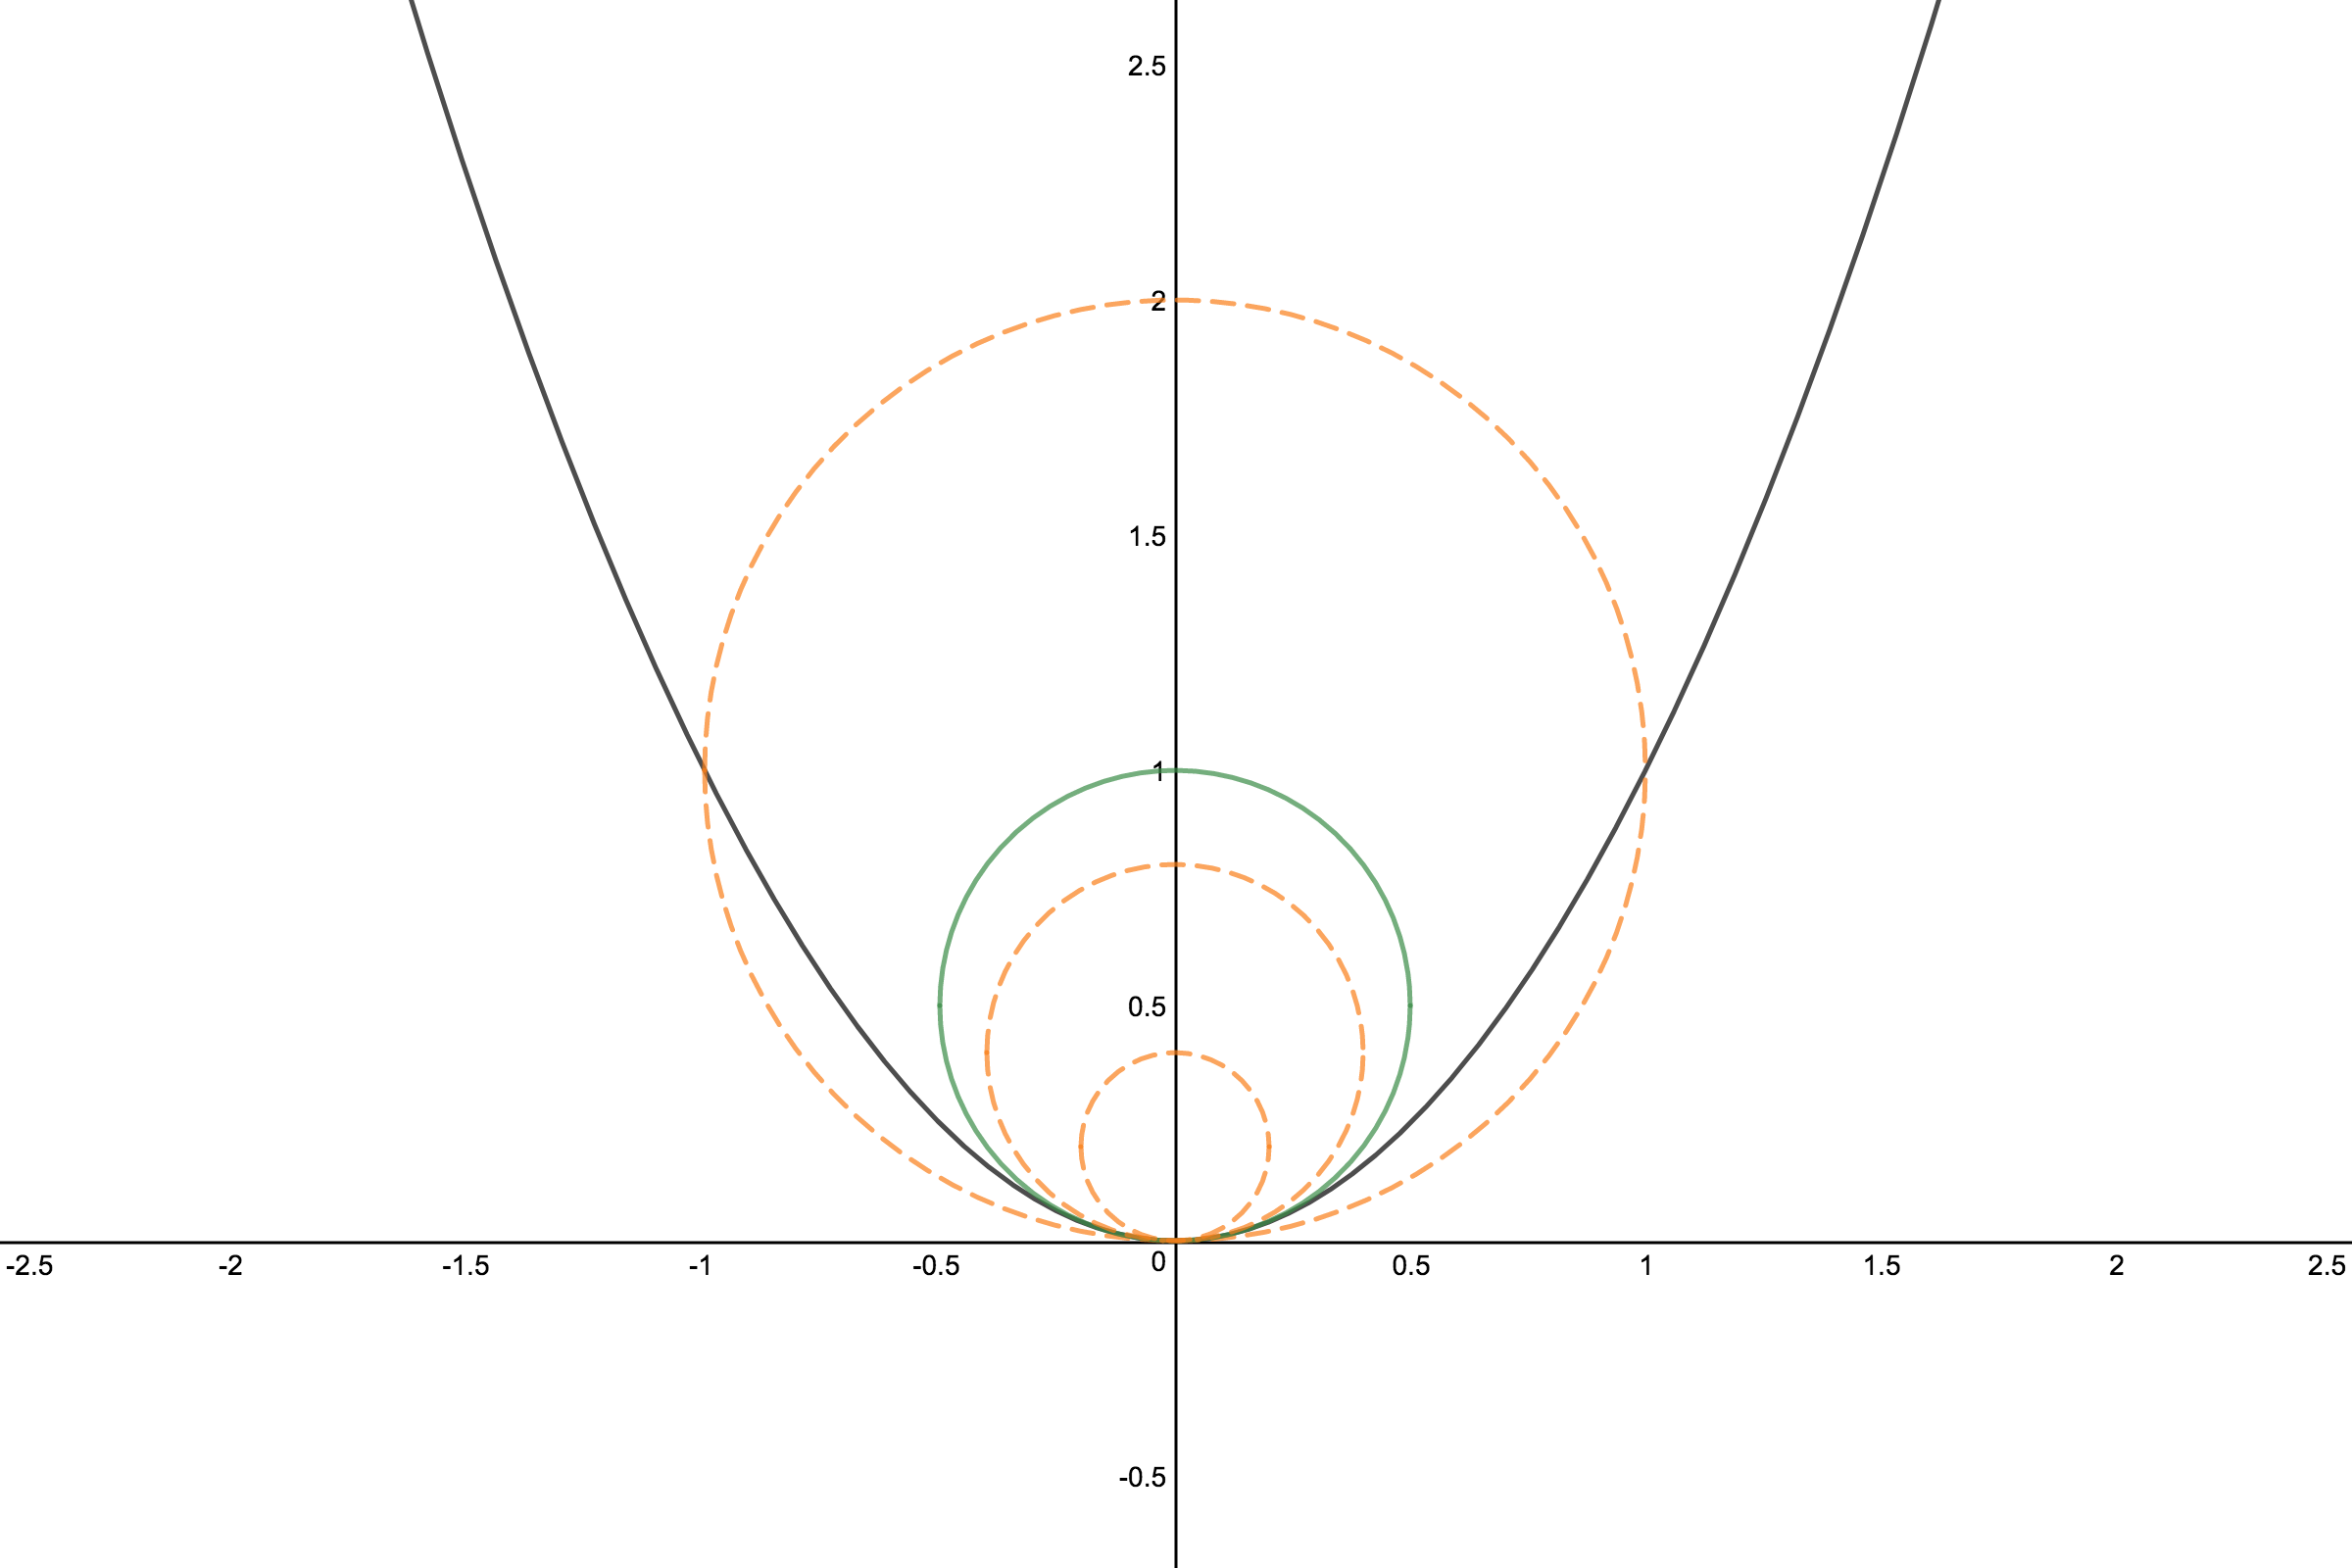
\includegraphics[height=9cm]{parabola}
		\caption{A circle of radius $1/2$ best approximates the parabola $y=x^2$ at $x=0$.}
\end{figure}
\begin{figure}[H]
		\centering
		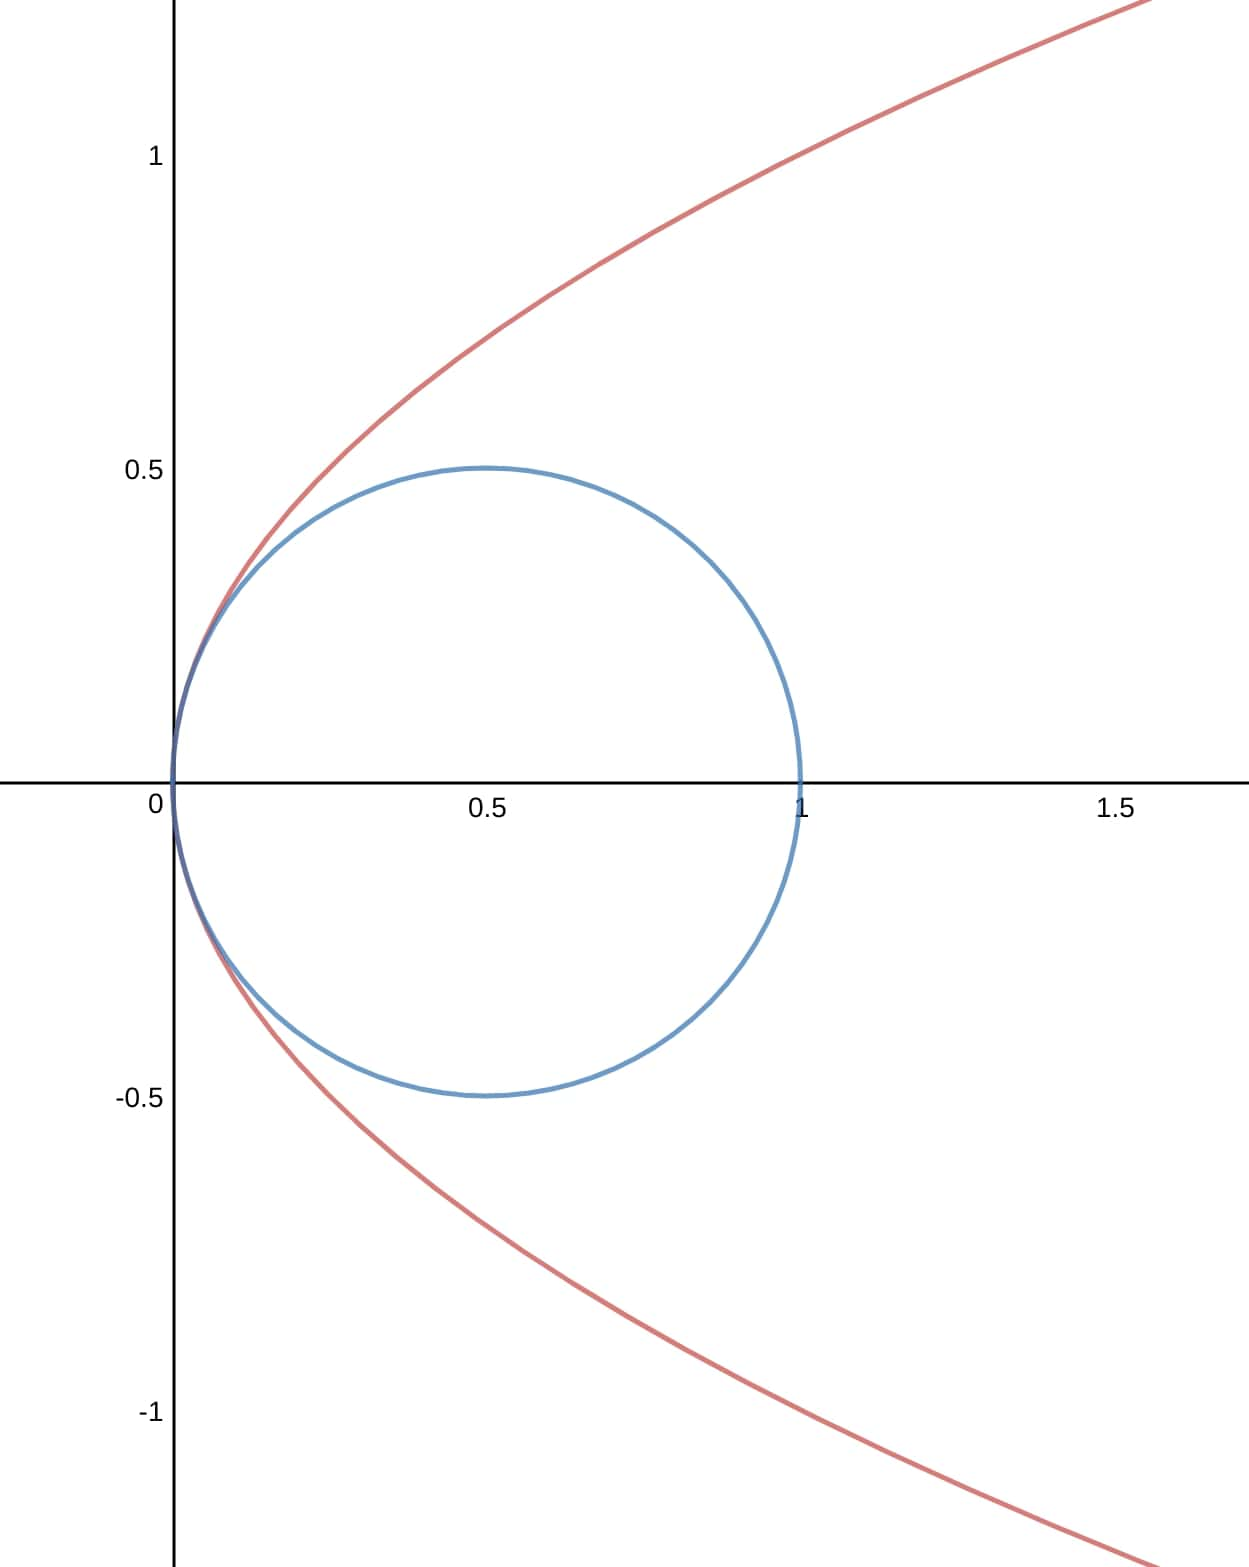
\includegraphics[height=9cm]{horizontal_parabola}
		\caption{Even if our curve is not a graph the same interpretation remains true.}
\end{figure}
